\documentclass[crop,tikz]{standalone}
\usetikzlibrary{backgrounds}
\colorlet{blue}{cyan}
\tikzset{
  inverted/.style = {
    color=white,
    background rectangle/.style={fill},
    show background rectangle
  }
}

\usepackage{pgfplots}
\pgfplotsset{compat=1.18}

\pgfplotsset{
  inverted/.style = {
    every axis legend/.append style={
      draw=white,
      fill=black,
      text=white
    }
  },
}

\begin{document}
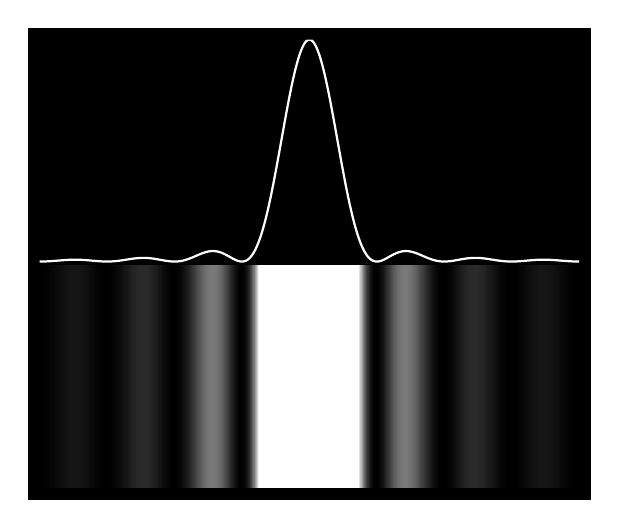
\begin{tikzpicture}[inverted,inverted]
  \pgfmathsetmacro{\maxz}{0.1}; % restrict z range to [0,\maxz]
  \begin{axis}[inverted,
    axis lines = none,
    view = {0}{90},
    xmin={-4*pi}, xmax={4*pi},
    ymin=0, ymax=2.02,
    zmin=0, zmax={\maxz},
    domain={-4*pi}:{4*pi},
    samples=1000,
    colormap={colorrange}{rgb=(0,0,0) rgb=(1,1,1)}, % color range from white to white
    ]
    \addplot[thick,smooth] (x,{1.02 + (sin(deg(x))/x)^2});
    \addplot3[surf,domain y=0:1,samples y=2,shader=flat,colormap name=colorrange] {min(\maxz,(sin(deg(x))/x)^2)};
  \end{axis}
\end{tikzpicture}
\end{document}
